\section{Konečné projektivní roviny}
\begin{t_definition}
  Konečná projektivní rovina je dvojice $(X, \mathcal{L})$, kde $X$ je konečná množina bodů a $\mathcal{L}\subseteq 2^X$ je množina přímek taková, že následující axiomy jsou splněny:
  \begin{enumerate}
    \item[(A1)]
    \textit{Každé dvě různé přímky se protínají v právě jednom bodě.}
    \\$\forall K,L\in\mathcal{L},K\neq L : |K\cap L|=1$
    \item[(A2)]
    \textit{Každé dva různé body určují právě jednu přímku.}
    \\$\forall x,y\in X,X\neq Y : \exists! L\in\mathcal{L} : \{x, y\}\subseteq L$
    \item[(A0)]
    \textit{Existuje čtveřice bodů taková, že žádné tři body z ní neleží na společné přímce.}
    \\$\exists Č\in\binom{X}{4}:\forall L\in\mathcal{L}:|Č\cap L|\leq 2$
  \end{enumerate}
\end{t_definition}

\begin{t_example}[Fanova rovina]$ $
  \begin{figure}[!htbp]
    \centering
    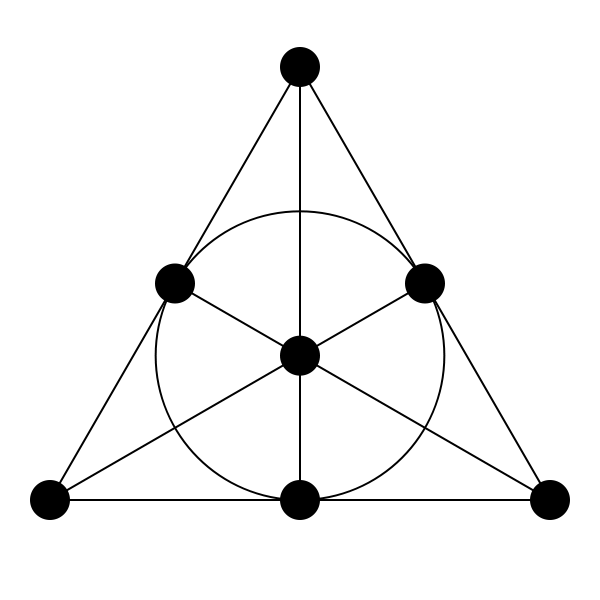
\includegraphics[width=0.5\textwidth]{img/fano_plane.png}
  \end{figure}
\end{t_example}

\begin{t_lemma}
  Nechť $(X, \mathcal{L})$ je konečná projektivní rovina, potom platí, že pro každou dvojici přímek existuje bod, který na nich neleží:
  \begin{align*}
    \forall K, L\in\mathcal{L} : \exists x\in X : x\notin K\cup L
  \end{align*}
\end{t_lemma}
\begin{t_proof}
  Uvažme množinu $Č$ za axiomu (A0) a libovolné dvě různé přímky $K, L\in\mathcal{L}$. Podle axiomu (A0) musí platit, že $K$ i $L$ každá protíná nejvýše 2 body z $Č$. Ekvivalentně zapsáno $|K\cap Č|\leq 2$ a $|L\cap Č|\leq 2$. To znamená, že $|(K\cup L)\cap Č|\leq 4$.
  
  Rozlišíme dva případy:
  \begin{enumerate}
    \item Pokud $|(K\cup L)\cap Č|\leq 3$, musí existovat alespoň jeden bod z $Č$, který nenáleží $K$ ani $L$. Vybereme tedy libovolný bod $x\in Č\setminus(K\cup L)$.
    \item Pokud $|(K\cup L)\cap Č|= 4$, je zřejmé, že $K$ a $L$ má v $Č$ právě dva průsečíky, označme je $K\cap Č=\{a,b\}$ a $L\cap Č=\{c,d\}$.
    
    Zaveďme označení $\overline{xy}$ pro přímku určenou body $x$ a $y$. Doplníme, že podle (A2) musí vždy taková přímka existovat a musí být určena jednoznačně až na pořadí bodů. Jednoduché pozorování je, že $\overline{ab}$ je $K$ a $\overline{cd}$ je $L$.
    
    Podle (A1) musí mít přímky $\overline{ac}$ a $\overline{bd}$ průsečík $x=\overline{ac}\cap\overline{bd}$. Víme ale také, že bod $x$ nemůže ležet na $K$, protože by přímka $K$ měla spolu s přímkami $\overline{ac}$, $\overline{bd}$ dvojice průsečíků $\{a,x\}$ a $\{b,x\}$, což by porušilo axiom (A1). Analogicky bod $x$ nemůže ležet ani na $L$.
    
    Bod $x$ tedy má vlastnost, kterou jsme hledali, a důkaz je dokončen.
  \end{enumerate}
\end{t_proof}

\begin{t_theorem}
  Nechť $(X, \mathcal{L})$ je konečná projektivní rovina, potom platí, že každá přímka protíná stejný počet bodů. Ekvivalentně:
  \begin{align*}
    \forall K, L\in\mathcal{L}:|K|=|L|
  \end{align*}
\end{t_theorem}

\begin{t_proof}
  Uvažme libovolné dvě přímky $K, L\in\mathcal{L}$. Podle předchozího lemmatu musí existovat bod $x\in X$, který na nich neleží. Můžeme zavést zobrazení $f:K\rightarrow L$ definované tak, že obrazem bodu $t$ je průsečík přímky $\overline{xt}$ a $L$, formálněji: $f(t)=\overline{xt}\cap L$. 
  
  Nyní ukážeme, že $f$ je bijekce, z čehož vyplývá, že přímky $K$ a $L$ mají stejný počet bodů. Aby zobrazení $f$ bylo vzájemně jednoznačné, musí být zároveň prosté a na. 
  \begin{itemize}
    \item
    Zobrazení $f$ je prosté, protože pokud by existovaly dva body $t_1, t_2\in K$ takové, že $f(t_1)=f(t_2)=s$, znamenalo by to, že přímky $\overline{xt_1}$ a $\overline{xt_2}$ mají dva průsečíky $\{x,s\}$, což je spor s axiomem (A1).
    
    \item
    Zobrazení $f$ je na, protože každý bod $s\in L$ určuje podle axiomu (A2) přímku $\overline{xs}$, která podle axiomu (A1) musí mít průsečík $t\in K$.
  \end{itemize}
\end{t_proof}

\begin{t_definition}
  Řád konečné projektivní roviny $(X,\mathcal{L})$ je $|L|-1$, kde $L\in\mathcal{L}$.
\end{t_definition}

\begin{t_example}
  Fanova rovina je rovinou řádu 2, protože každá přímka protíná právě 3 body.
\end{t_example}

\begin{t_theorem}
  Nechť $(X,\mathcal{L})$ je konečná projektivní rovina řádu $n$. Potom platí:
  \begin{enumerate}
    \item
    \textit{Každým bodem prochází $n+1$ přímek.}
    \\$\forall x\in X:|\{L\in\mathcal{L}\mid x\in L\}| = n+1$
    
    \item
    $|X|=n^2+n+1$
    
    \item
    $|\mathcal{L}|=n^2+n+1$
  \end{enumerate}
\end{t_theorem}

\begin{t_proof}
  \begin{enumerate}
    \item
    Uvažme libovolný bod $x\in X$ a přímku $L\in\mathcal{L}$, která jej neobsahuje. Podle předchozí věty musí přímka $L$ obsahovat právě $n+1$ bodů. Tyto body, spolu s bodem $x$, určují podle axiomu (A2) právě $n+1$ různých přímek. Nyní víme, že bodem $x$ prochází alespoň $n+1$ přímek. Nemůžeme si ale být jisti, že jich není více.
    
    Pokud by taková situace nastala, znamenalo by to, že přímka $L$ by s těmito přímkami musela mít společných více než $n+1$ bodů (spor s řádem roviny) nebo by některé z těchto přímek musely protínat stejný bod vícekrát (alespoň dvě přímky mají dva průsečíky). V každém případě bychom došli ke sporu. Bodem $x$ tedy musí procházet právě $n+1$ přímek.
    
    \item
    Uvažme opět stejnou situaci s bodem $x\in X$ a přímkou $L\in\mathcal{L}$, která jej neobsahuje. Na $L$ leží právě $n+1$ bodů, které spolu s bodem $x$ určují $n+1$ různých přímek, označme je $\mathcal{K}=\{K_1, K_2,\dots K_{n+1}\}$.
    
    Na každé přímce $K_i\in\mathcal{K}$ musí ležet také $n+1$ bodů. Víme, že jedním z těchto bodů je bod $x$, který sdílejí všechny přímky z $\mathcal{K}$. Zbylých $n$ bodů na přímce $K_i$ již nemůže ležet na žádné další přímce z $\mathcal{K}$, protože by každý další bod společný dvěma přímkám z $\mathcal{K}$ byl po bodu $x$ jejich druhým průsečíkem, což by porušilo axiom (A1).
    
    V $\mathcal{K}$ tedy musí být vyjma bodu $x$ celkem $(n+1)n=n^2+n$ různých bodů. Přidáme-li k tomuto počtu bod $x$, získáme $n^2+n+1$ bodů, což jsme chtěli dokázat. Úvahu uzavřeme pozorováním, že každý bod z $L$ náleží právě jedné přímce z $\mathcal{K}$ a kromě bodů přímek z $\mathcal{K}$ se v rovině žádný další bod vyskytovat nemůže, jinak by došlo k porušení axiomu (A1). Tím je důkaz hotov.
    
    \item
    Důkaz tohoto bodu je analogický k bodu 2. a vyplývá z duality bodů a přímek v konečných projektivních rovinách.
  \end{enumerate}
\end{t_proof}

\begin{t_definition}
  Množinový systém je dvojice $(X,\mathcal{L})$, kde $X$ je konečná množina a $\mathcal{L}\subseteq 2^X$. Množinu $X$ nazýváme nosnou množinou systému $(X,\mathcal{L})$.
\end{t_definition}

\begin{t_remark}
  Pozorujeme, že každá konečná projektivní rovina je množinovým systémem, ale ne všechny množinové systémy jsou konečnými projektivními rovinami.
\end{t_remark}

\begin{t_example}
  Nechť je $X=\{1,2,3\}$ a $\mathcal{L}=\{\{1,3\},\{1,2\},\{3\}\}$. $(X,\mathcal{L})$ je množinový systém.
\end{t_example}

\begin{t_definition}
  Pro každý množinový systém $(X,\mathcal{L})$ definujeme incidenční graf $(V,E)$, kde $V=X\cup\mathcal{L}$ a $E=\{(x,L)\mid x\in X, L\in\mathcal{L}, x\in L\}$.
\end{t_definition}

\begin{t_remark}
  Incidenční graf množinového systému je bipartitní graf, jehož jedna partita je tvořena prvky nosné množiny a druhá partita množinami v systému. Hrany spojují prvky nosné množiny s množinami v systému, ve kterých jsou tyto prvky obsaženy.
\end{t_remark}

\begin{t_remark}
  Axiomy konečných projektivních rovin je možno interpretovat geometricky na incidenčních grafech. Rozmyslete si, jak by vypadalo jejich znění.
\end{t_remark}

\begin{t_definition}
  Multimnožina je množina, ve které se každý prvek může vyskytnout víckrát než jednou. Můžeme jí jednoduše zkonstruovat pomocí obyčejné množiny a zobrazení, které každému prvku z množiny přiřadí jeho četnost v multimnožině.
\end{t_definition}

\begin{t_example}
  Multimnožinu $\tilde{X}=\{e_1, e_2, e_3, e_2, e_2, e_3\}$ zkonstruujeme použitím obyčejné množiny $X=\{e_1, e_2, e_3\}$ a zobrazení $f:X\rightarrow\mathbb{N}$ takového, že $f(e_1)=1$, $f(e_2)=3$ a $f(e_3)=2$.
\end{t_example}

\begin{t_remark}
  Dále v textu bude každá množina považována za multimnožinu.
\end{t_remark}

\begin{t_definition}
  Pro každý množinový systém $(X,\mathcal{L})$ definujeme jeho duální systém $(Y,\mathcal{M})$ tak, že jejich incidenční grafy jsou isomorfní po výměně partit. Přesněji, $Y=\mathcal{L}$, $\mathcal{M}=\{M_x\mid x\in\mathbb{X}\}$, kde $M_x=\{L\in\mathcal{L}\mid x\in L\}$.
\end{t_definition}

\begin{t_theorem}
  Duální systém konečné projektivní roviny je konečnou projektivní rovinou stejného řádu.
\end{t_theorem}

\begin{t_proof}
  Mějme konečnou projektivní rovinu $(X,\mathcal{L})$ a její duální systém $(Y,\mathcal{M})$. Aby $(Y,\mathcal{M})$ byl konečnou projektivní rovinou, musí splňovat všechny tři axiomy z definice. Pozorujeme, že axiom (A1) v $(X,\mathcal{L})$ implikuje platnost axiomu (A2) v $(Y,\mathcal{M})$. Stejně tak axiom (A2) v $(X,\mathcal{L})$ implikuje platnost axiomu (A1) v $(Y,\mathcal{M})$. Zbývá ověřit platnost axiomu (A0).
  
  Jestliže v $(X,\mathcal{L})$ existuje čtveřice bodů taková, že žádné tři z nich neleží na jedné přímce, potom musí existovat i čtveřice přímek taková, že žádné tři z nich nemají společný průsečík. Tím je dokázána platnost axiomu (A0) v $(Y,\mathcal{M})$.
\end{t_proof}

\begin{t_corollary}
  Každé tvrzení o konečné projektivní rovině může být díky této dualitě převedeno na jiné ekvivalntní tvrzení.
\end{t_corollary}

\begin{t_theorem}
  Nechť je $n$ mocninou prvočísla, $\mathbb{K}$ těleso s $n$ prvky a $\mathbb{K}^3$ vektorový prostor dimenze 3 nad $\mathbb{K}$, potom existuje konečná projektivní rovina řádu $n$.
\end{t_theorem}

\begin{t_proof}
  Definujeme relaci $\sim$ na $\mathbb{K}$ tak, že $x\sim y\equiv \exists\lambda\in\mathbb{K}, \lambda\neq 0:x=\lambda y$. Nahlédneme, že relace $\sim$ je ekvivalence, pojďme nyní prozkoumat její třídy na $\mathbb{K}^3\setminus 0$. Jejich reprezentanty jsou tyto vektory:
  \begin{itemize}
    \item $(1,\alpha,\beta)$, kde $\alpha,\beta\in\mathbb{K}$ – těchto vektorů je $n^2$,
    \item $(0,1,\alpha)$, kde $\alpha,\in\mathbb{K}$ – těchto vektorů je $n$,
    \item $(0,0,1)$ – pouze jeden vektor.
  \end{itemize}
  
  Vektory budou množinou bodů $X=\mathbb{K}^3\setminus 0$. Pro každý vektor $x\in X$ definujeme přímku $L_x=\{y\in X\mid x\cdot y=0\}$, takto získáme $n^2+n+1$ přímek, které seskupíme v množině $\mathcal{L}=\{L_x\mid x\in X\}$. Aby $(X,\mathcal{L})$ byla konečnou projektivní rovinou, musí splnit axiomy.
  \begin{enumerate}
    \item[(A1)] Máme dvě přímky $L_a, L_b$ a zajímá nás počet bodů, které mají společné. Body $y$ v $L_a$ musí splňovat $a\cdot y=0$, body v $L_b$ musí splňovat $b\cdot y=0$. Společné body obou přímek jsou řešením soustavy těchto dvou rovnic.
    
    Je triviální nahlédnout, že uvedená soustava má vždy právě jedno řešení.
    
    \item[(A2)] Analogickou úvahou.
    
    \item[(A0)] ... % todo
  \end{enumerate}
\end{t_proof}

\begin{t_exercise}
  \item Dokažte, že axiom (A0) můžeme v definici KPR nahradit axiomem (A0a):\\
  \textit{Existují 2 přímky takové, že každá z nich má alespoň 3 body.}
  \\$\exists K, L\in\mathcal{L}:|K|\geq 3\wedge|L|\geq 3$
  
  \item Dokažte, že axiom (A0) můžeme v definici KPR nahradit axiomem (A0b):\\
  \textit{Neexistují 2 přímky takové, že by pokryly všechny body.}
  \\$\forall K, L\in\mathcal{L}:K\cup L\subset X$
  
  \item Pokuste se nakreslit konečnou projektivní rovinu řádu 3.
  
  \item Ukažte, že až na isomorfismus je Fanova rovina jedinou projektivní rovinou řádu 2.
  
  \item Dokažte, že pro nekonečně mnoho různých $n$ existují grafy na $n$ vrcholech s $\Omega(n^\frac{3}{2})$ hranami, které neobsahují jako podgraf $C_4$. Ke konstrukci můžete využít konečné projektivní roviny.
\end{t_exercise}